\section{Thực nghiệm và đánh giá}
\subsection{Dữ liệu và giao thức chung}
\label{sec:protocol}
Nhóm thực nghiệm trên năm cơ sở dữ liệu chuẩn (benchmark, bộ dữ liệu dùng để so
sánh thuật toán) của cộng đồng FIM: Chess, Mushroom, Retail, T10I4D100K và
Accidents, đều có nguồn gốc từ kho FIMI~\cite{fimi}. Bảng~\ref{tab:datasets} liệt kê các thống kê
do nhóm tự tính từ chính các tệp dữ liệu, trong đó $N$ là số giao dịch, $|I|$ là
số item phân biệt, $\bar{w}$ là độ dài giao dịch trung bình và mật độ
$d = \bar{w} / |I|$ là tỉ lệ item trung bình có mặt trong một giao dịch. Chess và
Mushroom là dữ liệu dày đặc (dense, $d \ge 0{,}19$), còn Retail và T10I4D100K là
dữ liệu thưa (sparse, $d \le 0{,}012$). Accidents nằm giữa hai nhóm với
$d = 0{,}072$, nhưng lớn nhất cả về số giao dịch lẫn độ dài giao dịch.

\begin{table}[t]
\centering
\caption{Thống kê năm benchmark, tính từ tệp đã kiểm tra SHA-256}
\label{tab:datasets}
\begin{tabular}{lrrrrr}
\hline
Dữ liệu & $N$ & $|I|$ & $\bar{w}$ & $w_{\max}$ & $d$ \\
\hline
Chess & 3\,196 & 75 & 37,00 & 37 & 0,493 \\
Mushroom & 8\,124 & 119 & 23,00 & 23 & 0,193 \\
Retail & 88\,162 & 16\,470 & 10,31 & 76 & 0,0006 \\
T10I4D100K & 100\,000 & 870 & 10,10 & 29 & 0,0116 \\
Accidents & 340\,183 & 468 & 33,81 & 51 & 0,072 \\
\hline
\end{tabular}
\end{table}

Mỗi tệp được định danh bằng mã băm SHA-256 thay vì bằng tên, vì cùng một tên có
thể ứng với nhiều phiên bản khác nhau. Bản \texttt{mushrooms.txt} trên SPMF có
8\,416 giao dịch, khác với bản 8\,124 giao dịch của FIMI mà đề bài và đa số bài
báo sử dụng, nên nhóm dùng bản của FIMI. Retail là các hóa đơn ẩn danh của một cửa
hàng bán lẻ ở Bỉ~\cite{brijs1999}, còn Accidents là hồ sơ tai nạn giao thông có
người bị thương ở vùng Flanders, Bỉ~\cite{geurts2003}; bản Chess và Accidents trên
SPMF giống hệt bản của FIMI từng byte. Retail và T10I4D100K của FIMI
chứa item 0 trong khi SPMF chỉ nhận item nguyên dương, nên nhóm dùng bản của SPMF,
trong đó mọi mã item được cộng thêm 1. Phép đổi tên này giữ nguyên support của
mọi itemset. Kịch bản \texttt{experiments/prepare\_benchmarks.jl} tải lại dữ liệu,
kiểm tra mã băm và thống kê trước khi đưa tệp vào sử dụng.

Ngưỡng support tối thiểu tương đối minsup được đổi thành số giao dịch
$\sigma = \lceil \mathrm{minsup} \cdot N \rceil$. Khi đo thực nghiệm, nhóm phát
hiện SPMF tính phép nhân này bằng số thực dấu phẩy động 64 bit, nên với
$\mathrm{minsup} = 0{,}07$ và $N = 100$, SPMF yêu cầu $\sigma = 8$ trong khi phép
tính thập phân chính xác cho $\sigma = 7$. Vì vậy, trình chạy thực nghiệm từ chối
mọi ngưỡng mà hai cách tính cho kết quả khác nhau, để sai lệch giữa hai cài đặt
chỉ có thể đến từ thuật toán.

Mọi lần chạy (attempt) diễn ra trong một tiến trình (process) mới, có giới hạn
thời gian (timeout) và được ghi thành các dòng CSV với cùng một tập trường: dữ
liệu và mã băm, minsup và $\sigma$, revision Git, phiên bản thuật toán, môi trường,
seed, thời gian, bộ nhớ đỉnh, số itemset và trạng thái. Lần chạy lỗi hoặc quá
thời gian vẫn được giữ lại với trạng thái tương ứng, không bao giờ được thay bằng
giá trị 0. Thời gian được tách theo phạm vi đo (timing scope): \emph{process} đo
toàn bộ tiến trình, gồm cả khởi động Julia, biên dịch JIT (just-in-time, biên dịch
khi chạy) hoặc khởi động JVM; \emph{mine} đo riêng lời gọi \texttt{mine} sau khi
đã chạy khởi động (warm-up) trên một cơ sở dữ liệu nhỏ, nên không chứa thời gian
biên dịch. Với SPMF, nhóm dùng thêm thời gian do SPMF tự báo cáo. Bộ nhớ đỉnh là
peak RSS (resident set size, lượng bộ nhớ vật lý lớn nhất mà tiến trình chiếm) do
hệ điều hành đo, vì chỉ đại lượng này so sánh được giữa tiến trình Julia và Java.

Loạt đo thời gian của nhóm chạy trên máy AMD Ryzen 7 H 260 (16 luồng logic, 31,3 GiB RAM),
Windows 11, Julia 1.13.2 với một luồng, SPMF v2.66~\cite{spmf2016} trên Java
Temurin 25.0.4.1.
\subsection{Độ đúng và bộ nhớ}
Để kiểm tra độ đúng, chúng tôi chạy Eclat của SPMF như chương trình tham chiếu
độc lập. Bộ so sánh đọc toàn bộ ánh xạ từ tập mục phổ biến (frequent itemset)
sang độ hỗ trợ (support), chuẩn hóa thứ tự mục rồi đối chiếu từng cặp. Tỉ lệ
khớp là số tập mục có cùng độ hỗ trợ trong cả hai đầu ra chia cho số tập mục
khác nhau trong hợp của hai đầu ra. Ánh xạ trống ở cả hai phía được tính là
khớp hoàn toàn. Một tập mục xuất hiện hai lần trong cùng một đầu ra không được
tính là khớp, vì khi đó độ hỗ trợ của nó không xác định.

Bảng~\ref{tab:toy-spmf} trình bày kết quả trên bảy cơ sở dữ liệu nhỏ. $N$ là
số giao dịch; $\sigma$ là ngưỡng hỗ trợ theo số giao dịch như ở
Mục~\ref{sec:protocol}. Cột ``Khớp'' ghi số tập mục có cùng độ hỗ trợ với SPMF
trên tổng số tập mục khác nhau. Mỗi phép so sánh của bản cơ bản đạt 100\%,
không có tập mục thiếu, thừa, lặp hoặc sai độ hỗ trợ; với \texttt{disjoint},
cả hai chương trình đều trả về ánh xạ trống. Cơ sở dữ liệu \texttt{boundary}
được chạy ở hai ngưỡng để kiểm tra tập mục vừa nằm trên và dưới ngưỡng. Mỗi
ngưỡng được chọn sao cho SPMF và phép tính thập phân cho cùng $\sigma$. Đầu ra
gốc của SPMF và danh sách lần chạy nằm trong \texttt{data/toy/spmf/}, kèm kịch
bản \texttt{tools/spmf/reference\_outputs.jl} để tạo lại. Bộ kiểm thử đối chiếu
các đầu ra này với mọi phiên bản Eclat ở mỗi lần chạy. Giao thức nằm trong
\texttt{tools/spmf/README.md}.

\begin{table}[t]
\centering
\caption{Đối chiếu toàn bộ tập mục và độ hỗ trợ của bản Eclat cơ bản với SPMF
trên cơ sở dữ liệu nhỏ.}
\label{tab:toy-spmf}
\begin{tabular}{lrrr}
\hline
Dữ liệu & $N$ & $\sigma$ & Khớp \\
\hline
Baskets & 4 & 2 & 6/6 \\
Duplicates & 3 & 2 & 3/3 \\
Disjoint & 3 & 2 & 0/0 \\
Dense & 2 & 2 & 7/7 \\
Groceries & 5 & 2 & 5/5 \\
Boundary & 4 & 2 & 2/2 \\
Boundary & 4 & 1 & 4/4 \\
Nested & 4 & 2 & 3/3 \\
\hline
\end{tabular}
\end{table}
\subsubsection{Đối chiếu trên năm benchmark}
Nhóm chạy cả bản cơ bản và bản tối ưu từ revision \texttt{8c043fb} trên
33 cặp dữ liệu và ngưỡng trong cấu hình \texttt{correctness.toml}.
Hai biến thể dùng chung một đầu ra SPMF Eclat cho từng cặp. Cả 66 phép so sánh
đều đạt 100\%, với 0 tập mục thiếu, thừa, lặp hoặc sai support.
Bảng~\ref{tab:bench-exact} ghi số điểm khớp theo biến thể và khoảng số itemset
trong đầu ra tham chiếu. Kết luận áp dụng cho các tệp và ngưỡng đã chạy.

\begin{table}[t]
\centering
\caption{Số điểm benchmark khớp toàn bộ ánh xạ với SPMF Eclat.}
\label{tab:bench-exact}
\begin{tabular}{lrrr}
\hline
Dữ liệu & Cơ bản & Tối ưu & Khoảng số itemset \\
\hline
Chess & 7/7 & 7/7 & 622--254\,944 \\
Mushroom & 7/7 & 7/7 & 153--574\,431 \\
Retail & 6/6 & 6/6 & 159--7\,589 \\
T10I4D100K & 6/6 & 6/6 & 385--96\,959 \\
Accidents & 7/7 & 7/7 & 15--1\,093 \\
\hline
\end{tabular}
\end{table}

\subsubsection{Bộ nhớ đỉnh của tiến trình}
Loạt đối chiếu và loạt đo bộ nhớ dùng máy AMD Ryzen 5 6600H, Windows 11,
Julia 1.13.2 với một luồng, và SPMF 2.66 trên Temurin 25.0.4.1. Mỗi bộ dữ liệu
được đo tại một ngưỡng giữa đã khớp SPMF. Mỗi biến thể chạy trong năm tiến trình
mới. Windows báo \texttt{PeakWorkingSetSize} qua \texttt{GetProcessMemoryInfo}.
Phép đo bao gồm khởi động, đọc dữ liệu, khai thác và ghi toàn bộ đầu ra. Phép
đối chiếu diễn ra sau khi đo. Cả 50 đầu ra đo bộ nhớ đều khớp SPMF.

\begin{table}[t]
\centering
\caption{Trung vị peak RSS trên năm lần lặp. RSS được ghi theo MiB.}
\label{tab:peak-rss}
\begin{tabular}{lrrrr}
\hline
Dữ liệu & $\sigma$ & Cơ bản & Tối ưu & $R$ \\
\hline
Chess & 2\,397 & 217,5 & 193,7 & 1,123 \\
Mushroom & 2\,031 & 216,8 & 188,4 & 1,151 \\
Retail & 221 & 229,2 & 215,1 & 1,065 \\
T10I4D100K & 100 & 253,4 & 218,4 & 1,160 \\
Accidents & 272\,147 & 582,2 & 466,9 & 1,247 \\
\hline
\end{tabular}
\end{table}

\begin{figure*}[t]
\centering
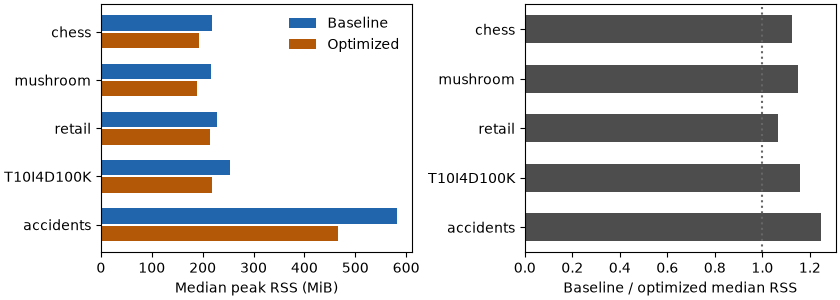
\includegraphics[width=0.88\textwidth]{figures/peak-memory.png}
\caption{Trung vị peak RSS theo bộ dữ liệu và tỷ lệ bộ nhớ giữa hai biến thể.}
\label{fig:peak-rss}
\end{figure*}

Trong Bảng~\ref{tab:peak-rss} và Hình~\ref{fig:peak-rss}, $R$ là trung vị RSS
của bản cơ bản chia cho trung vị RSS của bản tối ưu. Bản tối ưu giảm peak RSS
ở cả năm điểm đo. Retail giảm 6,1\% và Accidents giảm 19,8\%. Peak RSS lớn nhất
của năm lần lặp Accidents là 627,6 MiB với bản cơ bản và 467,5 MiB với bản tối
ưu. Bản tối ưu tái sử dụng bitset cho các giao ở từng mức tìm kiếm. Cách tổ
chức này có thể giảm bộ nhớ của các danh sách tid trung gian, nhất là khi các
danh sách chứa nhiều giao dịch. Các phép đo tiến trình không tách riêng phần
bộ nhớ của tidset khỏi dữ liệu đầu vào, đầu ra và runtime. Vì vậy tỷ lệ $R$
được dùng để mô tả bộ nhớ toàn tiến trình tại các điểm đo này.

\subsection{Thời gian, số lượng kết quả và khả năng mở rộng}
Thien viết runtime/độ dài giao dịch; Hung viết output size và tập con lồng nhau
10\%, 25\%, 50\%, 75\%, 100\%. Dẫn chiếu hình và dữ liệu thô khi có kết quả.
\subsection{Phân tích và hướng phát triển}
Thien đề xuất ít nhất hai tối ưu tương lai dựa trên bottleneck đã đo; phân biệt
với kỹ thuật tối ưu Hung đã thực hiện trong chương cài đặt.
